\clearpage
\item \subquestionpoints{5}
For Dataset 1, create a plot of the validation set with $x_1$ on the horizontal
axis, and $x_2$ on the vertical axis. To visualize the two classes, use a
different symbol for examples $x^{(i)}$ with $y^{(i)} = 0$ than for those with
$y^{(i)} = 1$. On the same figure, plot the decision boundary found by logistic
regression in part (b). Make an identical plot with the decision boundary found
by GDA in part (e).

\ifnum\solutions=1 {
\begin{answer}

\begin{figure}[h]
    \centering
    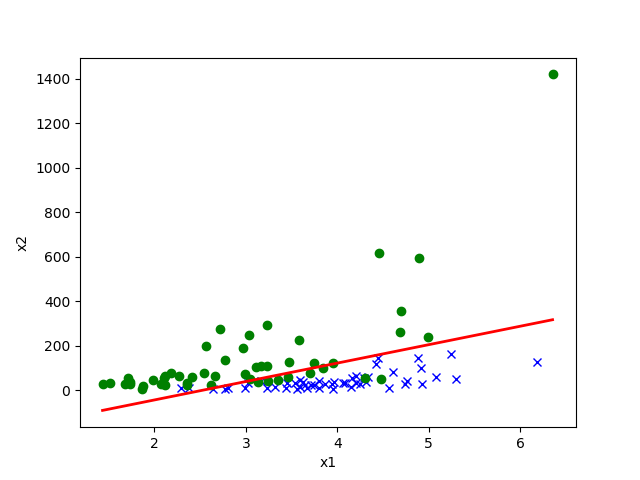
\includegraphics[width=0.6\textwidth]{p01b_pred_1_txt_lr_valid}
    \caption{Logistic Regression on Dataset 1}
\end{figure}

\begin{figure}[h]
    \centering
    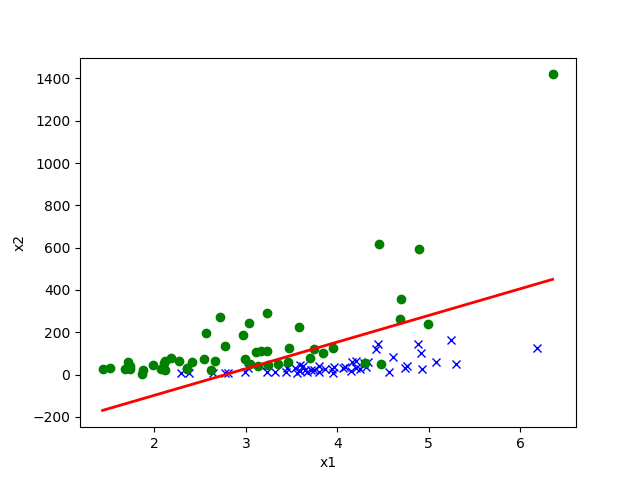
\includegraphics[width=0.6\textwidth]{p01e_pred_1_txt_gda_valid}
    \caption{GDA on Dataset 1}
\end{figure}
\end{answer}

} \fi
